Di seguito viene mostrata la pagina di avvio del software\ped{G}, viene inoltre mostrato come utilizzare i pulsanti presenti e come utilizzare le loro funzionalità con l'ausilio di immagini.

\subsection{Pagina iniziale}
La pagina iniziale si presenta come in figura.

\begin{figure}[H] 
	\centering 
	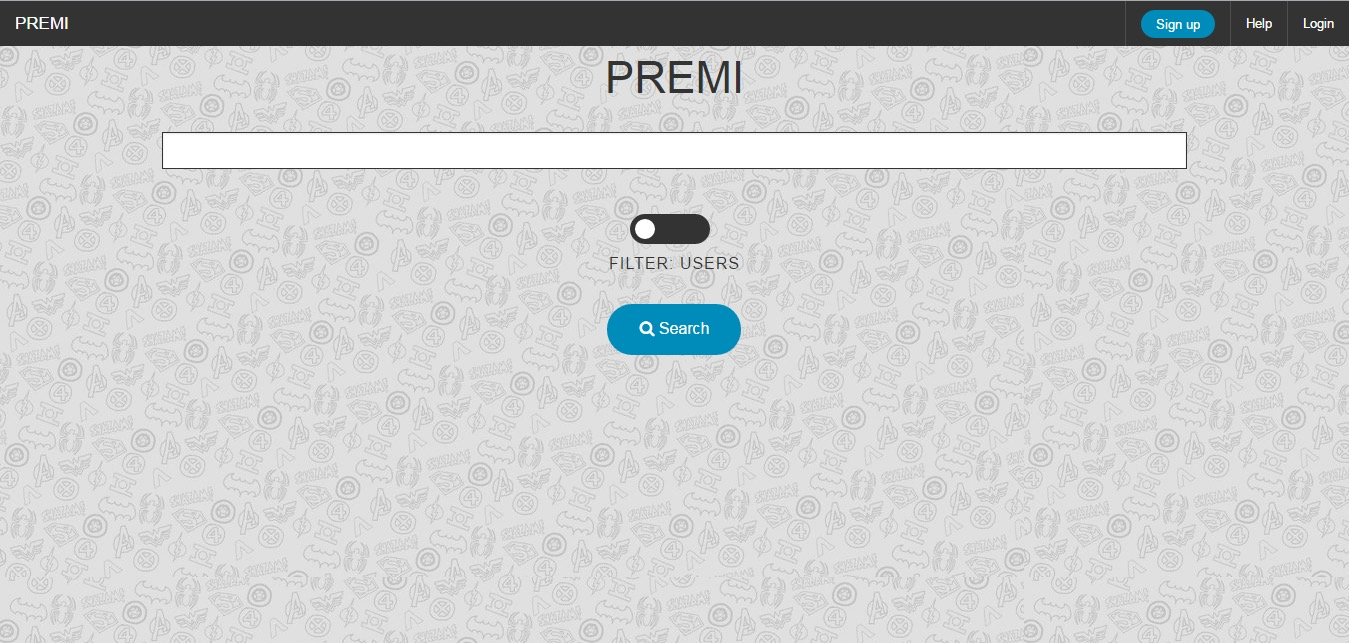
\includegraphics[scale=0.40] {img/pagina_iniziale}
	\caption{Pagina iniziale} 
\end{figure}

\noindent Nella parte in alto è presente una barra di colore nero con 4 pulsanti. Il pulsante \textit{PREMI} permette all'utente di tornare alla pagina iniziale in qualsiasi momento. Il pulsante \textit{Sign Up} permette ad un utente di registrarsi al sito. Il pulsante \textit{Help} permette all'utente di visualizzare il manuale utente. Il pulsante \textit{Login} permette ad un utente già registrato di effettuare l'accesso al sito.
Nella parte centrale della pagina viene visualizzato il nome dell'applicativo \textbf{PREMI}, sotto ad esso si trova la barra adibita alla ricerca con annesso il filtro per la ricerca e il pulsante \textit{Search} che permette di avviare la ricerca. Tutte le funzionalità di tali pulsanti sono esplicitate nelle sezioni seguenti.

\subsection{Registrazione}
Per creare un nuovo account utente è necessario premere il pulsante \textbf{Sign Up} posto nell'angolo superiore destro dello schermo. Si aprirà un pop-up\ped{G} nel quale saranno richieste le informazioni necessarie per registrare il nuovo utente (tutti i campi dati sono obbligatori). Dopo aver inserito i propri dati è sufficiente premere il tasto \textbf{Confirm}.

\begin{figure}[H] 
	\centering 
	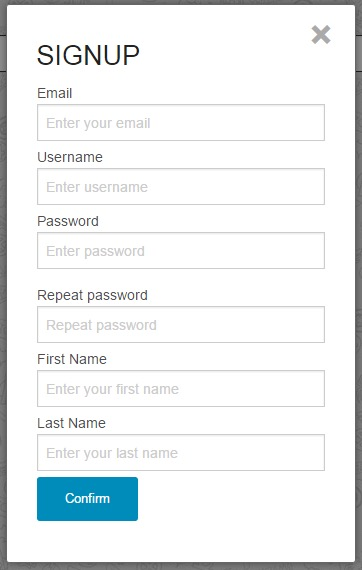
\includegraphics[scale=0.40] {img/signup}
	\caption{Registrazione} 
\end{figure}


\noindent Nel caso in cui tutti i dati inseriti siano stati accettati, il sistema effettuerà in automatico il login del nuovo utente creato reindirizzandolo alla sua pagina personale.
In caso contrario verranno segnalati i campi dati da correggere.

\subsection{Autenticazione}
Se un utente è già in possesso di un account e vuole autenticarsi è necessario premere il pulsante \textbf{Login} posto nell'angolo superiore destro dello schermo, infine inserire il proprio username, la password e premere \textbf{OK}.

\begin{figure}[h] 
	\centering 
	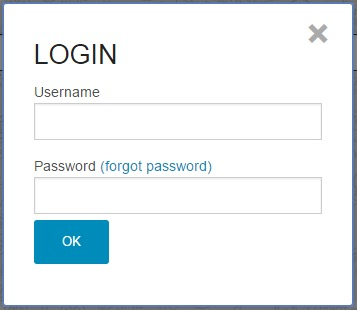
\includegraphics[scale=0.40] {img/login}
	\caption{Login} 
\end{figure}

\noindent Se i dati inseriti sono corretti il sistema reindirizzerà l'utente alla propria pagina personale, altrimenti verrà segnalato un errore nelle credenziali inserite.



\noindent Nel caso in cui l'utente non ricordi più la sua password, può premere il link \textit{Forgot password}. Una volta premuto si aprirà un pop-up\ped{G} nel quale verrà richiesto di inserire la mail utilizzata al momento della registrazione al fine di recuperare la password di accesso. Dopo aver inserito la mail corretta e aver premuto \textbf{Submit} la procedura di recupero password sarà inviata alla mail indicata. Il pop-up\ped{G} è mostrato nella figura sottostante.

\begin{figure}[H] 
	\centering 
	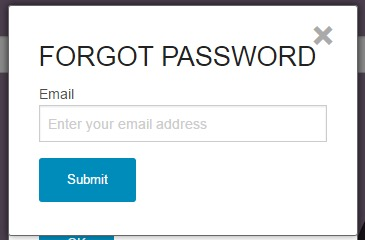
\includegraphics[scale=0.40] {img/forgot}
	\caption{Recupero password} 
\end{figure}

\subsection{Pagina personale}
Una volta autenticato, l'utente ha accesso alla sua pagina personale, nella quale sono riportati tutti i dati relativi a esso e dalla quale può accedere a tutte le funzionalità del sistema.

\begin{figure}[H] 
	\centering 
	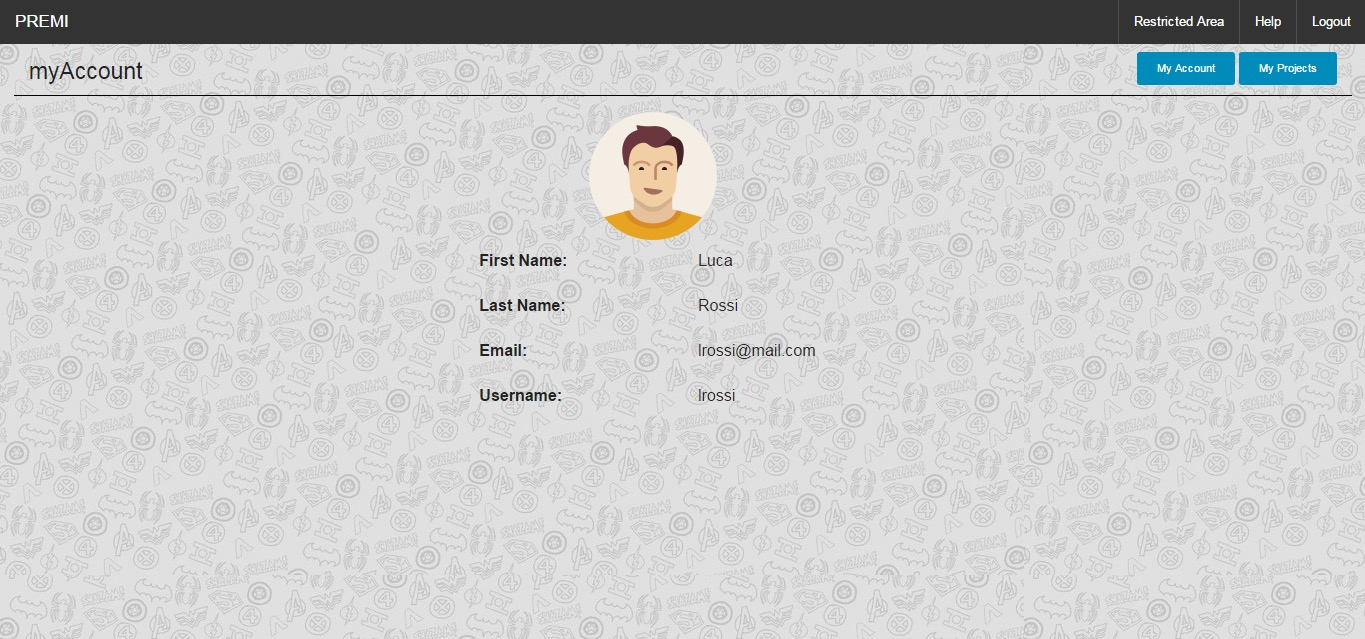
\includegraphics[scale=0.40] {img/MyAccount}
	\caption{Pagina personale} 
\end{figure}

\subsection{Logout}
Un utente autenticato può eseguire il logout, da qualunque pagina stia visualizzando, tramite il pulsante \textbf{Logout} posto nell'angolo in alto a destra dello schermo.

\begin{figure}[H] 
	\centering 
	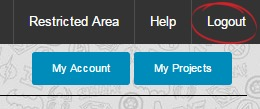
\includegraphics[scale=0.80] {img/logout}
	\caption{Logout} 
\end{figure}
